% !TeX spellcheck = sk_SK-Slovak
\documentclass[a4paper]{article}
\usepackage[slovak]{babel}
\usepackage[utf8]{inputenc}
\usepackage[T1]{fontenc}
\usepackage{a4wide}
\usepackage{amsmath}
\usepackage{amsfonts}
\usepackage{amssymb}
\usepackage{mathrsfs}
\usepackage[small,bf]{caption}
\usepackage{subcaption}
\usepackage{xcolor}
\usepackage{graphicx}
\usepackage{enumerate}
\usepackage{hyperref}
\usepackage{fancyvrb}
\usepackage{listings}
%\usepackage{lstautogobble}
\usepackage{stmaryrd}

\lstset{basicstyle=\ttfamily,
	mathescape=true,
	escapeinside=||%,
	%autogobble
}


\fvset{tabsize=4}


\pagestyle{empty}
\setlength{\parindent}{0pt}

\newenvironment{modenumerate}
{\enumerate\setupmodenumerate}
{\endenumerate}

\newif\ifmoditem
\newcommand{\setupmodenumerate}{%
	\global\moditemfalse
	\let\origmakelabel\makelabel
	\def\moditem##1{\global\moditemtrue\def\mesymbol{##1}\item}%
	\def\makelabel##1{%
		\origmakelabel{##1\ifmoditem\rlap{\mesymbol}\fi\enspace}%
		\global\moditemfalse}%
}

\makeatletter
\def\@seccntformat#1{%
	\expandafter\ifx\csname c@#1\endcsname\c@section\else
	\csname the#1\endcsname\quad
	\fi}
\makeatother



\begin{document} 
	
\pagenumbering{arabic}
\pagestyle{plain}

\begin{center}
	\sc\large
	Formálne metódy tvorby softvéru\\
	Domáca úloha 5
\end{center}

Autor: Marián Kravec

\section{1.)}

V prípade, že nedovoľujeme strácanie správ to bolo pomerne priamočiare.

\begin{figure}[!h]
	\centering
	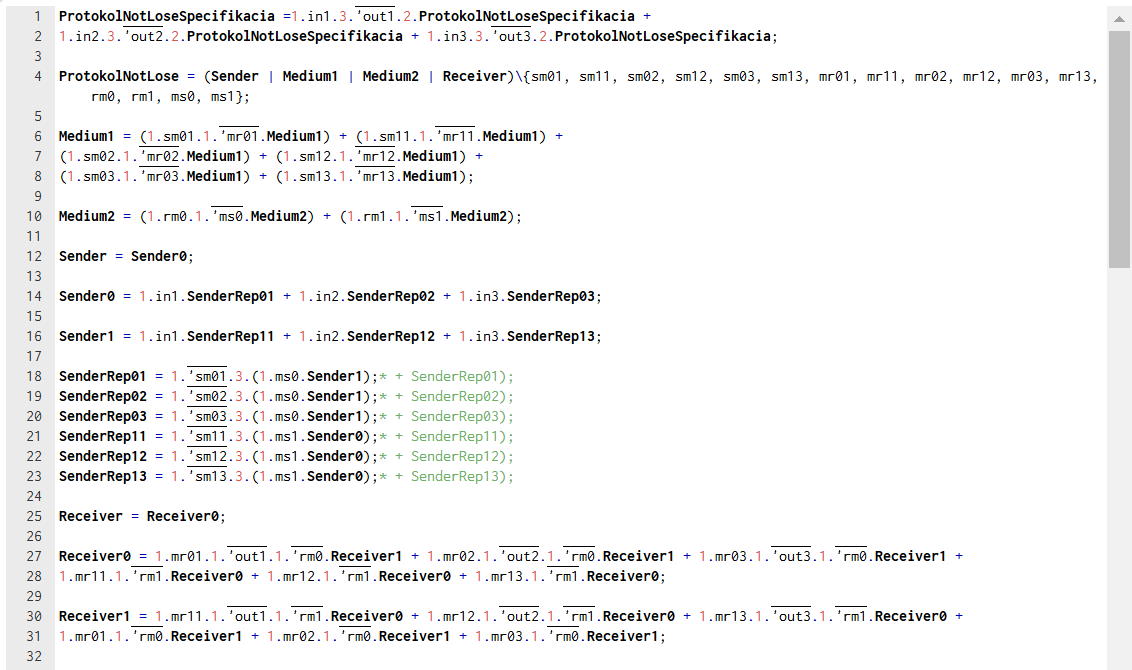
\includegraphics[width=1\textwidth]{lose_code.png}
	\caption{Kód ABP a špecifikácie}
\end{figure}

\begin{figure}[!h]
	\centering
	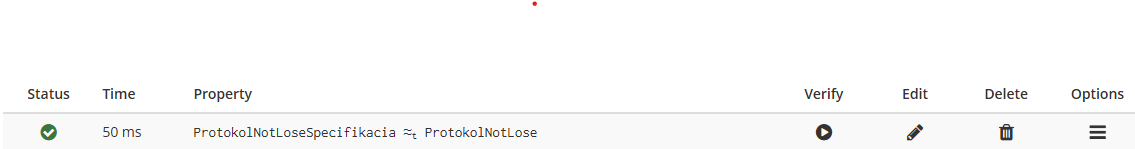
\includegraphics[width=1\textwidth]{lose_test.png}
	\caption{Kontrola slabej časovej bisimulácie}
\end{figure}
\newpage

\section{2.)}

V prípade, že dovoľujeme strácanie správ to bolo výrazne náročnejšie... Ja už netuším čomu zle rozumiem... čo robím zle... strácam nervy... určite sa na to ešte pred skúškou pozriem ale teraz na to fakt nemám energiu...

\begin{figure}[!h]
	\centering
	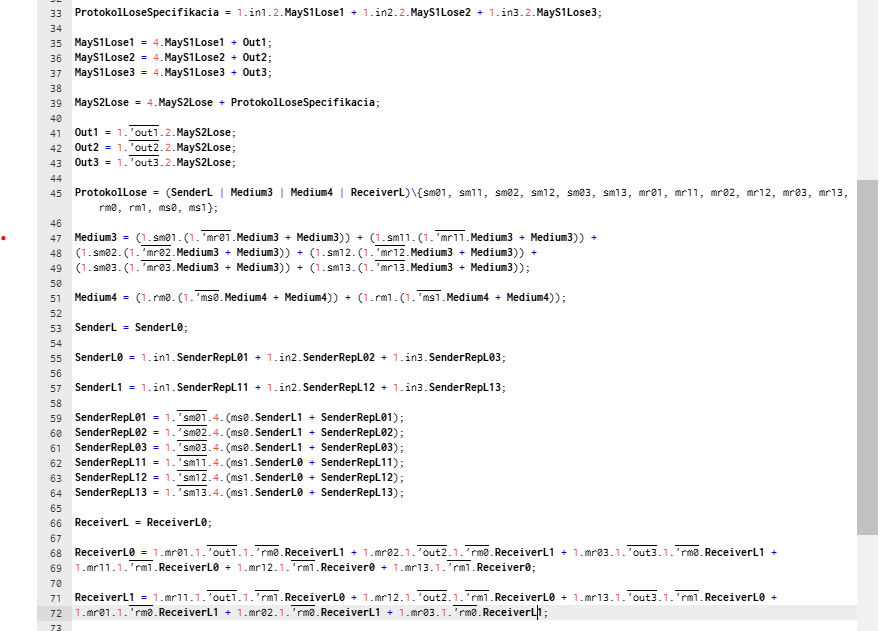
\includegraphics[width=1\textwidth]{lose_code_2.png}
	\caption{Kód ABP a špecifikácie}
\end{figure}

\begin{figure}[!h]
	\centering
	
\includegraphics[width=1\textwidth]{lose_test_2.png}
	\caption{Kontrola slabej časovej bisimulácie}
\end{figure}
\newpage

\section{3.)}

Keďže sa mi ORIS nepodarilo sfunkčniť, našiel som si systém PIPE (Platform Independent Petri net Editor) kde som si našiel príklad večerajúcich filozofov.

\begin{figure}[!h]
	\centering
	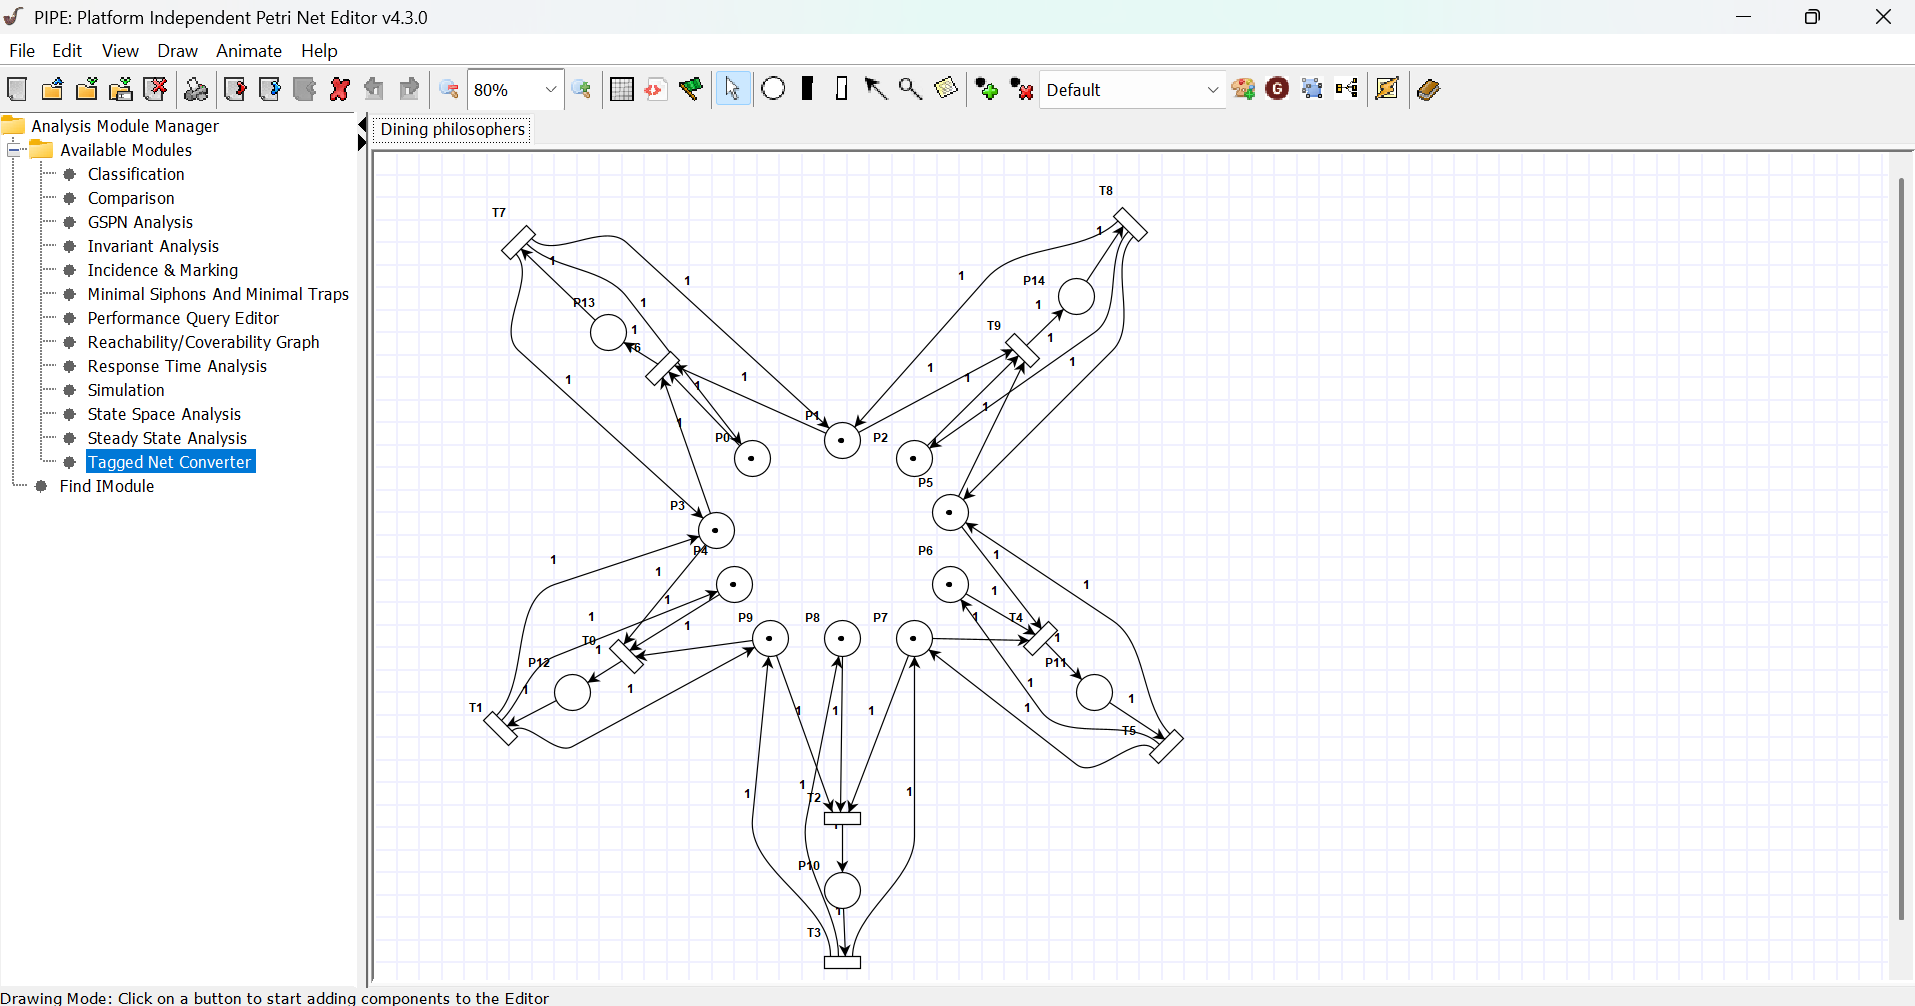
\includegraphics[width=1\textwidth]{dining_philo.png}
	\caption{Petriho sieť večerajúcich filozofov}
\end{figure}

Kde vidíme, že na to aby mohol filozof prejsť do stavu (place) je musí mať splnený 3 places, o dve sa delí s filozofmi okolo, jedna je len jeho, úplne mi nie je či place ktorý má filozof len pre seba má nejaký funkčný význam (myslím, že by to fungovalo aj bez neho) alebo iba má význam ako označenie že filozof je/neje (aj keď na to sa dajú použiť aj places ktoré sa aktivujú pri prechode do stavu je). Úplne neviem čo ďalej mám vysvetliť... Ak má filozof k dispozícii všetky 3 jeho places prejde do stavu je a potom eventuálne sa vráti späť a aktivuje svoje 3 places... Neviem to dobre vysvetliť... 

\end{document}